\section{Introduction}
\label{sec:intro}

Unmanned aerial vehicles (UAVs) have become an active area of research and have emerged as a pivotal technology for collecting data from distributed ground nodes (GNs)~\cite{lbc, assume, joint, Energy-Efficient-POI, msmo, DroneTank, Flight-Time-Minimization, AoI-Sensitive-Data-Collection, Cooperative-Data-Collection, Data-collection-and-offloading}.
GNs are widely deployed for environmental and infrastructure monitoring in settings such as bridges and railways, water, gas, and oil pipelines, and rivers and coastlines.
These GNs generate massive amounts of data that must be collected efficiently and periodically.
For example, Fig.~(\ref{fig:uav-data-collection-scenario}) illustrates a scenario in which sensors are deployed along a street in a city, and a UAV is dispatched to collect data from them by flying nearby and establishing line-of-sight (LoS) links. 

\begin{figure}
\centering
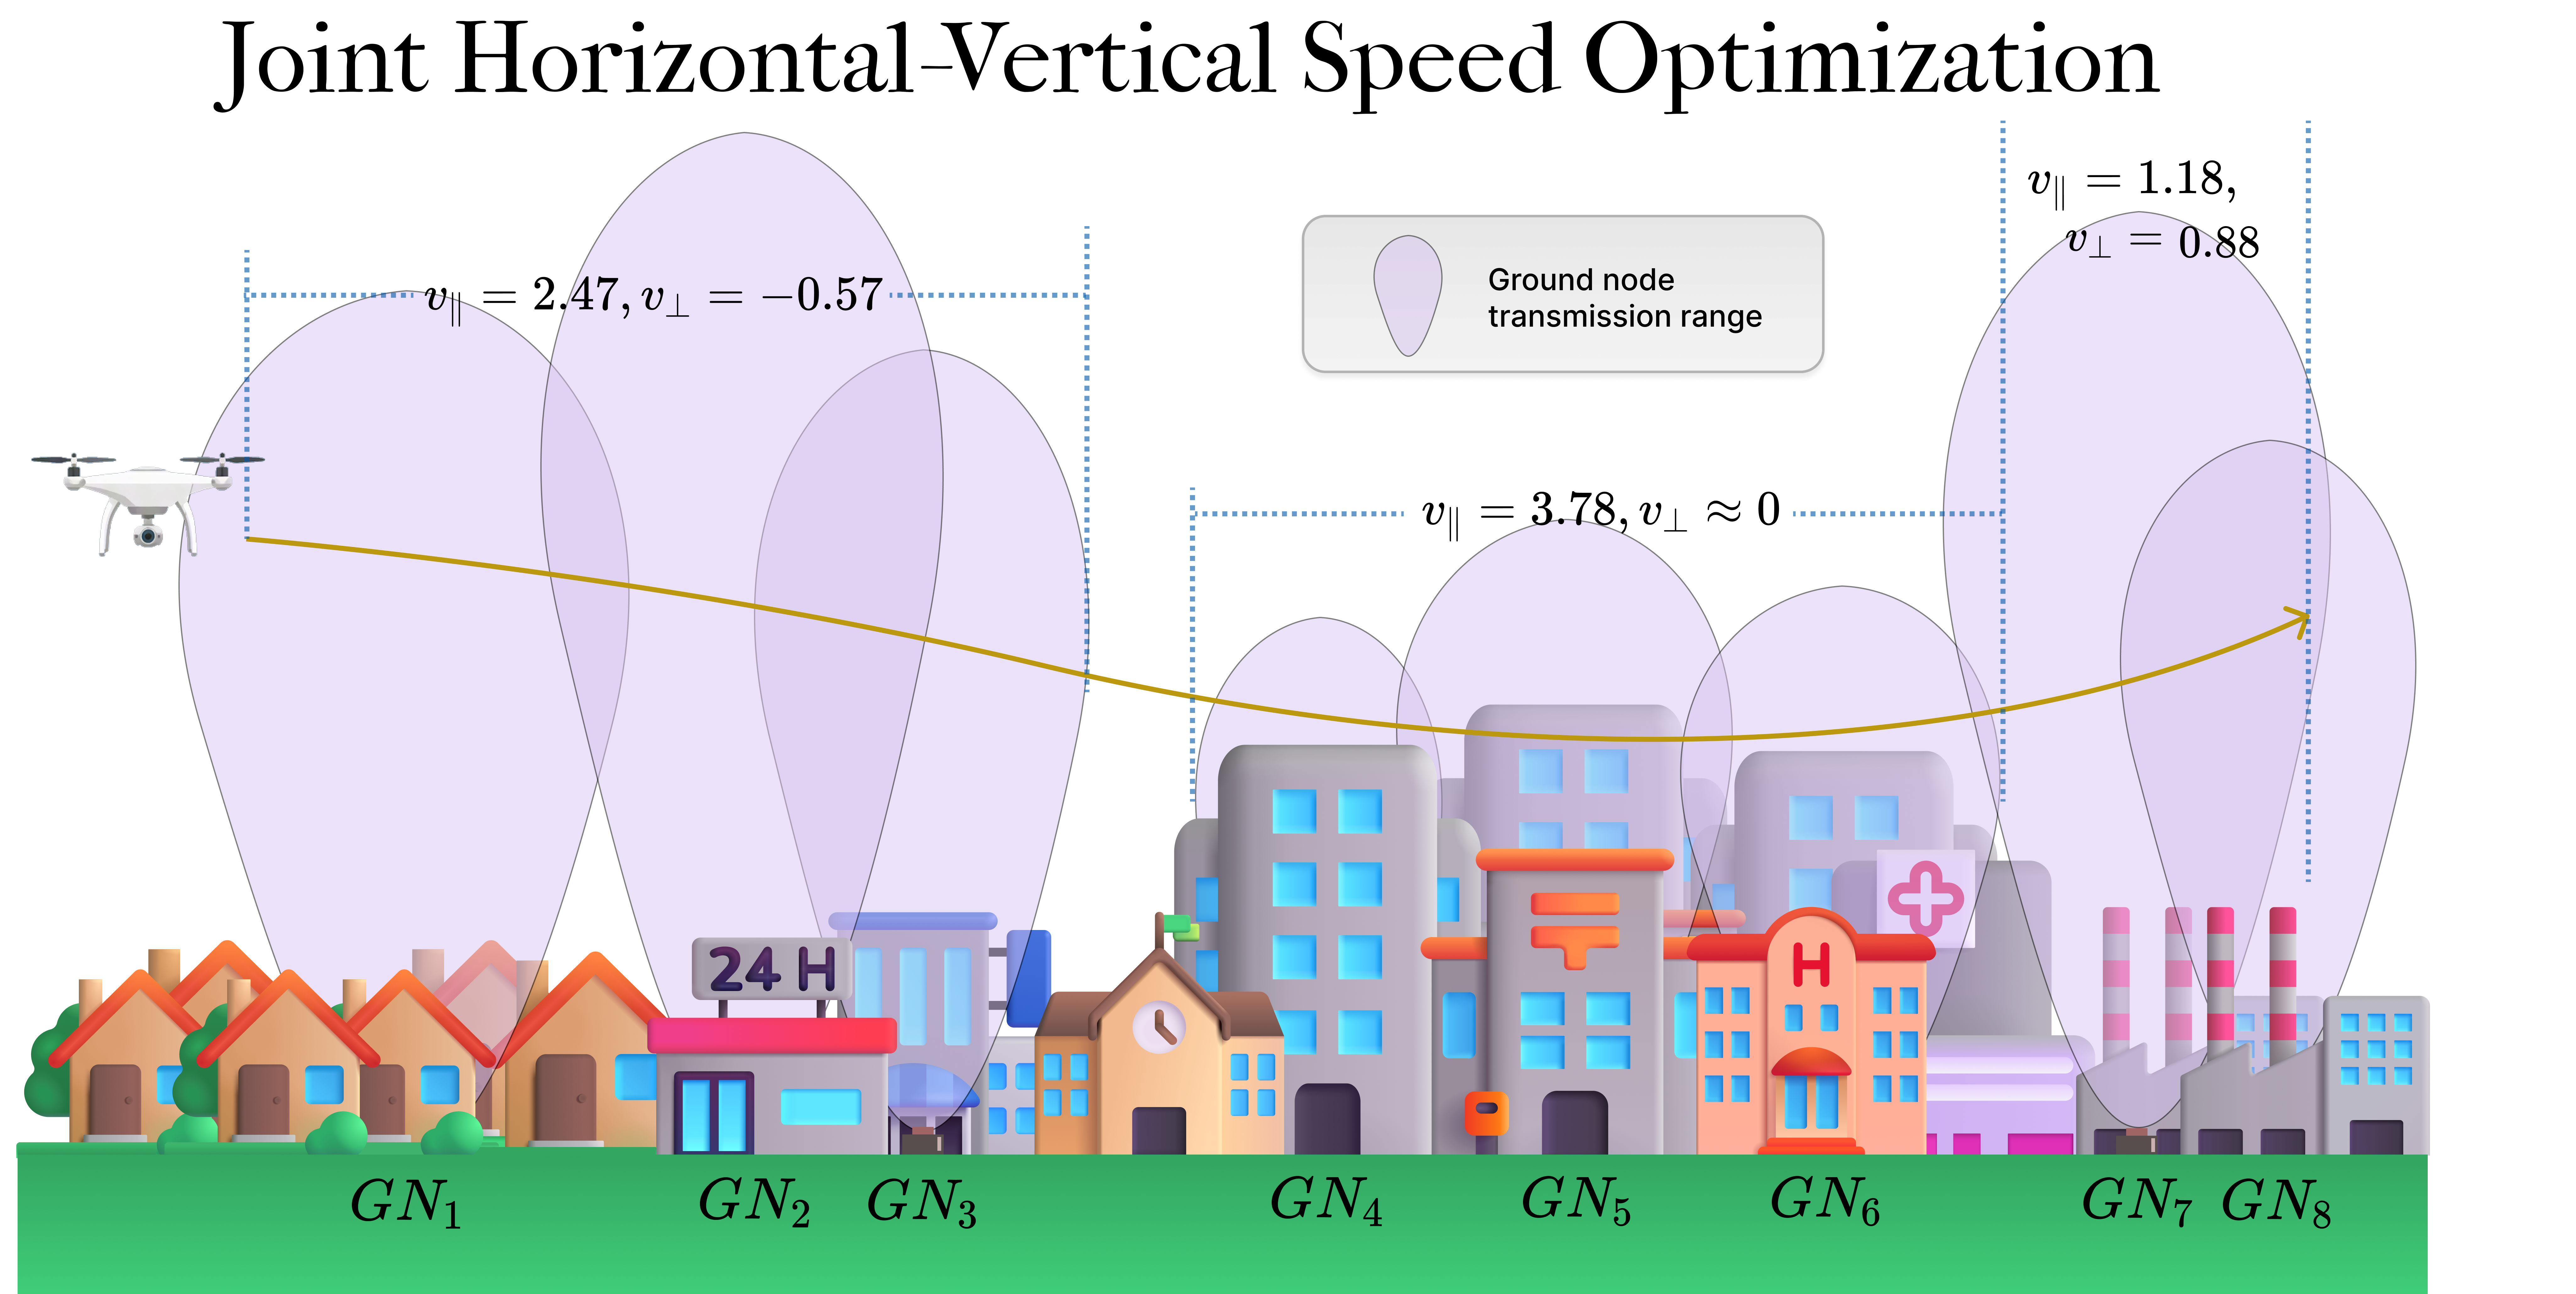
\includegraphics[width = 1\linewidth]{figures/figure1.png}
\caption{UAV-enabled data collection from distributed ground nodes (GNs) along linear infrastructure. A UAV flies along the deployment axis and collects data from each $GN_i$ through an altitude-dependent communication model (shaded cones), within which the UAV must remain for the required collection duration $\tau_i$. The horizontal speed $v_{\parallel}$ and vertical speed $v_{\perp}$ are jointly and continuously optimized so as to minimize the total flight energy while satisfying every GN's collection-time requirement.}
\label{fig:uav-data-collection-scenario}
\end{figure}

Given the inherent energy constraints of UAVs, optimizing flight trajectories to minimize energy consumption is critical~\cite{lbc, assume, joint}.
However, existing studies either concentrate on speed scheduling at a fixed height and restrict the vertical movement of UAVs~\cite{lbc}, or treat vertical movements independently as discrete transitions between horizontal segments~\cite{assume}.
In other words, the UAV's height is adjusted primarily for different horizontal sections rather than treated as a continuous variable in the optimization process~\cite{joint}.
In conclusion, in previous studies, the UAV's vertical movement is often treated independently or as discrete transitions between horizontal segments.

Distinct from previous works, we adopt a practical 3D flight energy consumption model.
Instead of optimizing horizontal speed and height separately, we focus on joint horizontal-vertical speed optimization.
Research has found that instantaneous flight power can be accurately calculated by summing the baseline hovering power with the independent power increments induced by the horizontal and vertical velocity components~\cite{GongHao, PowerConsumptionModel}.

Additionally, this paper assumes that the ground-to-air communication range varies with the UAV's flight height, which is more practical~\cite{assume}.
Although a higher height increases the probability of LoS, it may simultaneously reduce the communication coverage area of the UAV, which influences the level of energy minimization achieved. 
This observation motivates us to carefully optimize the horizontal and vertical speeds jointly to minimize the energy consumption for data collection.

Despite incorporating both the practical 3D flight energy consumption model and joint horizontal-vertical speed optimization, several challenges remain.

\begin{itemize}
\item 
GNs have different data collection volume requirements, which means that the UAV must fly at different speeds within the communication range of each GN to satisfy the required collection time.
Some communication ranges overlap, and the UAV collects data from only one GN at a time; therefore, the UAV must decide when to switch between GNs for data collection.

\item 
With our practical ground-to-air communication model, the communication range varies with height, which means that the UAV must also optimize the vertical component of its velocity.
An inappropriate vertical speed may cause the UAV to fly at an unsuitable height, resulting in a GN communication range that is too small or too large and thereby affecting the speed optimization.
However, the UAV's flight energy consumption is affected by the ascent or descent angle.

\item 
Minimizing the energy cost of data collection during UAV 3D speed optimization presents a further challenge.
On the one hand, the ascent or descent angle directly affects flight energy consumption.
On the other hand, flying faster or slower than a specific speed consumes more energy, as indicated by our practical flight energy consumption model.
How to balance the horizontal and vertical components of the UAV’s velocity while allowing the UAV sufficient time to collect all data at an appropriate height and minimizing flight energy consumption is a challenge.
\end{itemize}


To address this problem, we formulate a joint horizontal-vertical speed optimization problem under a practical 3D flight energy consumption model.
We first investigate its key optimality properties and establish several lemmas and theorems that provide the theoretical foundation for solving the problem.
We then develop an Optimal Reached Energy (ORE) dynamic programming algorithm by decomposing the trajectory into gap and task segments and recursively evaluating feasible transition states.
Finally, we conduct extensive simulations under various settings and a real-world case study to evaluate the energy efficiency and practical applicability of the proposed algorithm.
The major contributions of this paper are summarized as follows:

% contribution outline of the paper
% practical 3D flight energy consumption model
% joint horizontal-vertical speed optimization (JHVSO) problem 
% optimal reached energy (ORE) dynamic programming algorithm 

\begin{itemize}

\item
We formulate a joint horizontal--vertical speed optimization (JHVSO) problem for energy-efficient UAV data collection under a practical 3D flight energy consumption model.
Unlike previous formulations that optimize horizontal speed at a fixed height or schedule height separately, the JHVSO problem jointly considers horizontal and vertical motion, height-dependent communication ranges, and the required data collection time of each GN.

\item
We investigate the key optimality properties of the JHVSO problem and establish several lemmas and theorems that provide its theoretical foundation.
By exploiting the strict convexity of the horizontal and vertical flight energy functions, we prove that constant-velocity straight-line flight minimizes the energy between two states for a given duration.
We also derive the pitch-angle-dependent speed that minimizes the energy consumption per unit distance during unconstrained flight.

\item
We develop an Optimal Reached Energy (ORE) dynamic programming algorithm to solve the JHVSO problem.
By decomposing the UAV trajectory into gap and task segments, recursively evaluating feasible communication-boundary transition states, and establishing the non-aftereffect property between successive stages, the algorithm obtains the optimal local transition costs and \textbf{guarantees the global optimality} of the resulting solution over the discretized state space.

\item
We conduct extensive simulations under varying channel conditions, task durations, node densities, and inter-node distances to evaluate the proposed ORE algorithm.
The results show that the proposed JHVSO method consistently consumes less energy than ASSUME, MSMO, ACO, and a greedy speed--height baseline, achieving an energy reduction of up to approximately 16.8\% compared with the greedy speed--height baseline and by up to 5.8\% over the strongest competing baseline.
A case study involving 10 real-world traffic-camera locations further demonstrates its practical applicability.

\end{itemize}  

The remainder of this paper is organized as follows.
Section~\ref{sec:relatedworks} reviews the related works on energy-efficient UAV data collection and trajectory optimization.
Section~\ref{sec:systemmodel} introduces the system model and formulates the JHVSO problem.
Section~\ref{sec:problemanalysis} analyzes the problem and establishes the optimality properties required for its solution.
Section~\ref{sec:algorithm} presents the proposed ORE dynamic programming algorithm.
Section~\ref{sec:simulation} evaluates its performance through extensive simulations and a real-world case study.
Finally, Section~\ref{sec:conclusion} concludes the paper, and Appendices~\ref{pro:Lemma ver}--\ref{pro:Theorem optimal-range-speed} provide the relevant proofs.

%%%%%%%%%%%%%%%%%%%%%%%%%%%%%%%%%%%%%%%%%%%%%%%%%%%%%%%%%%%%%%%%%%%%%%%%%%%%%%%%%%
